\section{图像复原}
\label{sec:image_restoration}

图像复原是图像处理的另一重要课题,其主要目的 是改善给定图像的质量。当给定了一幅退化或受噪声污染的图像后,利用退 化现象的某种先验知识来重建或恢复原有图像是图 像复原处理的基本过程。这一部分以图像超分辨率重建为研究对象,对传统方法和基于深度学习的方法进行调研。

超分辨率图像重建利用已知的图像信息建立 LR图像与 HR 图像之间的特征序列关系,其数学模型为:利用``系统成像模型''自身的一些变化手段对退 化后的图像实现重建。``系统成像模型''过程:LR 图像由 HR 图像经退 化 函 数( 如 加 噪 、模 糊 、运 动 、降 采 样 等 )作 用 后 得 到 的不清晰图像,即:

\begin{equation}
\begin{aligned}
& D\left(I_{\mathrm{HR}} ; \theta_a\right)=\boldsymbol{S}_d \boldsymbol{B}_\kappa \boldsymbol{M} \boldsymbol{I}_{\mathrm{HR}}+n_{\xi}\{\boldsymbol{\kappa}, \xi, d\} \\
& I_{\mathrm{LR}}=D\left(I_{\mathrm{HR}} ; \theta_a\right)
\end{aligned}
\end{equation}

其中, $I_{\mathrm{LR}}$ 表示 LR 图像, $I_{\mathrm{HR}}$ 表示 $\mathrm{HR}$ 图像, $D$ 表示退 化函数, $\theta_a$ 表示与退化函数相关的各种参数和退化 因子, $S_d$ 为降采样矩阵, $d$ 为降采样矩阵的比例因 子, $\boldsymbol{B}$ 为模糊矩阵, $\kappa$ 为与 $\mathrm{HR}$ 卷积相关的模糊核, $\boldsymbol{M}$ 为运动矩阵, $n_{\xi}$ 为添加的带有标准差的噪声, $\xi$ 表示 标准差。

超分辨率图像重建问题为“系统成像模型”的逆 过程,输入 LR 图像重建出相应的 HR 图像:

\begin{equation}
I_{\mathrm{HR}}=R\left(I_{\mathrm{LR}} ; \sigma_a\right)
\end{equation}

其中, $R$ 表示重建函数, $\sigma_a$ 表示与重建函数相关的 各种参数与重建因子。图像退化过程和图像重建过程如 \textbf{图 \ref{fig:fig7}} 所示。黑色箭头表示图像退化过程,黄色箭头 表示图像重建过程。

\begin{figure}[!t]
\centering
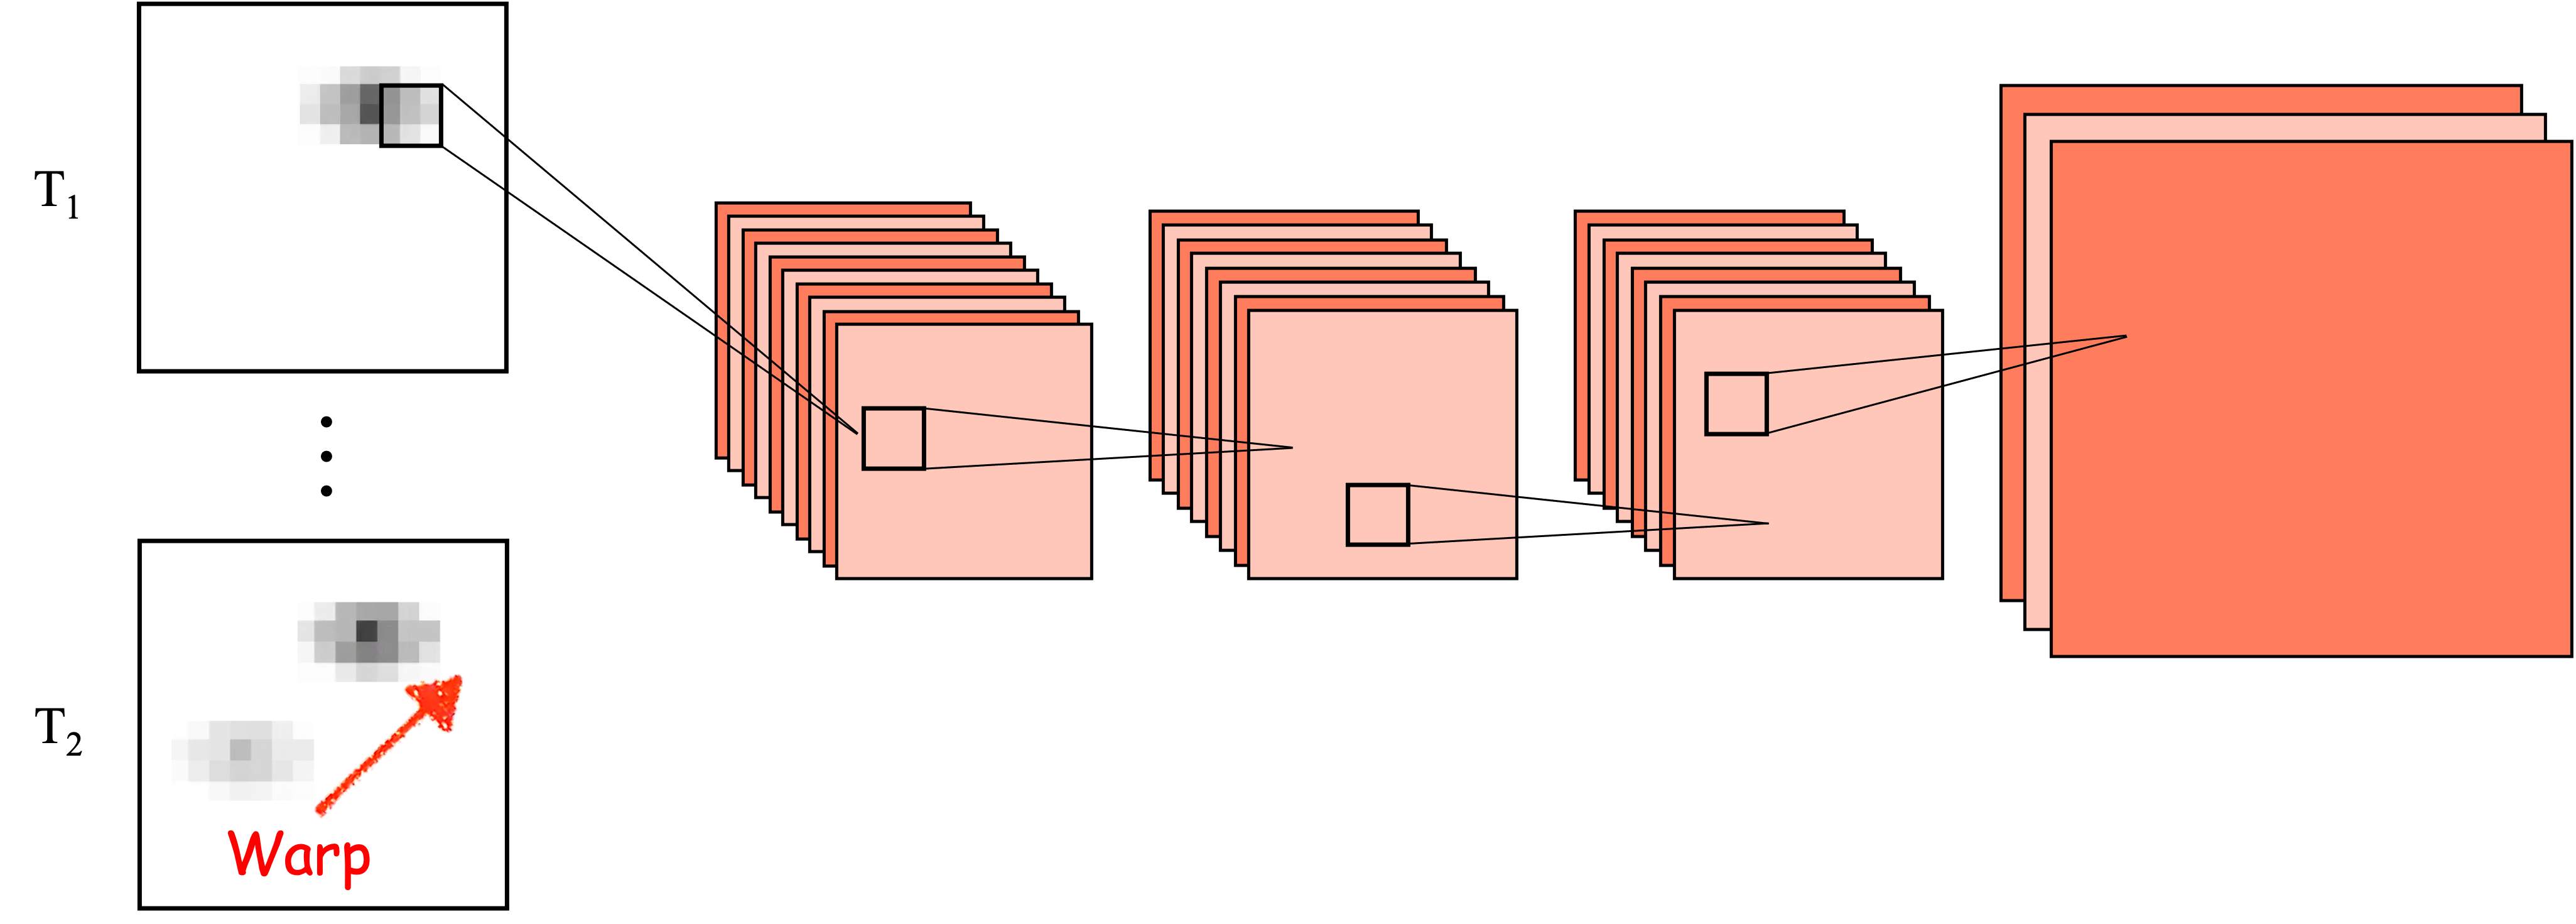
\includegraphics[width=\linewidth]{7.png}	
\caption{图像超分辨率重建技术图解}
\label{fig:fig7}
\end{figure}

\begin{figure*}[!b]
\centering
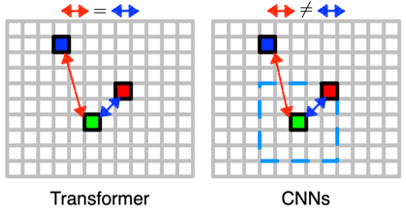
\includegraphics[width=\linewidth]{8.png}	
\caption{图像超分辨率重建方法分类}
\label{fig:fig8}
\end{figure*}


根据超分辨图像重建所采用的方法,将其 分为基于插值的图像重建方法、基于重构的图像重 建方法、基于学习的重建方法,而基于学习的图像重 建方法又可分为深度学习前的图像重建算法和深度 学习后的图像重建算法。深度学习后的图像重建算 法又分为基于卷积神经网络的超分辨率图像重建算 法、基于生成对抗网络的超分辨率图像重建算法和基于 Transformer 的超分辨率图像重建算法, 具体分类情况如 \textbf{图 \ref{fig:fig8}} 所示。本文将重点介绍基于插值的图像重建方法和基于卷积神经网络的深度学习图像重建方法。

\noindent\textbf{基于插值的图像重建方法}~基于插值的图像重建方法是超分辨率图像重建问题中最原始、最直观的方法,主要分为线性插值算 法和非线性插值算法。插值法主要根据 LR 图像已 知的像素点灰度信息,运用插值公式增强像素点间 的灰度信息来实现图像放大问题。一般情况下,插 值法所需的图像信息较少,算法复杂度较低,运行速 度较快,且插值后的 HR 图像保留了原 LR 图像的像 素点信息。基于插值的图像重建方法又包括线性插值算法和非线性插值算法两种。

\begin{enumerate}
	\item 线性插值算法
	\begin{itemize}
		\item \textbf{最近邻插值法}指插值点直接以与其欧式距 离最短的像素点的灰度值为自身插值后的灰度值。虽然它是最简单的插值算法,难度系数低且易实现, 但由于其他相邻像素点没有对目标插值点产生影 响,当插值图像分辨率较大时,容易出现锯齿效应和 图像灰度不连续问题。
		\item \textbf{双线性插值法}是为解决最近邻插值法忽视相邻像素点间影响而造成图像锯齿效应现象所提出的。双 线性插值法主要从垂直、水平两个方向对相邻的四 个像素点进行线性插值实现图像插值问题。虽然双 线性插值法在图像灰度不连续问题上有所改进,但 插值后的图像产生明显的细节退化,图像高频信息 受到损坏。
		\item \textbf{双三次插值法}是在双线性插值法的基础上提出的,将临近区域内四个相邻像素点扩充到十六个相邻像 素点,对其使用三次插值多项式后进行加权平均计 算完成图像插值重建。双三次插值法充分考虑了各 像素点对目标插值点的影响,提高了重建质量也使 计算变复杂,运算量急剧增加。
	\end{itemize}
	\item 非线性插值算法
	\begin{itemize}
		\item \textbf{边缘导向插值法}主要是对 RGB 三色图像的 边缘信息进行约束、放大,以便解决人眼视觉特性对 图像边缘信息的捕捉造成的影响。
		\item \textbf{梯度引导插值法}是利用邻域内一阶梯度、二 阶梯度的信息调整梯度分布和像素分布,再结合边 缘导向插值法和双三次线性插值法实现图像重建。
		\item \textbf{小波变换插值法}充分利用小波变换所具有 的局部细化特点,将图像特征信息分解到不同尺度 上独立研究与分析后,将提取的特征信息叠加融合 后再用小波逆变换提高图像分辨率。
	\end{itemize}
\end{enumerate}

\textbf{表 \ref{tab:tab1}} 给出了基于插值方法的各重建算法之间的 比较。基于插值的图像重建方法虽然简单且容易实 现,但图像重建效果并不理想。其中,单幅图像的重 建速度和重建效果尚且能够满足部分领域的需求, 但多幅图像的图像重建不能解决其在运算速度、运 算复杂度以及图像精度上所存在的问题。

\begin{table}[!ht]
\centering
\caption{基于插值的图像重建算法比较}
\begin{adjustbox}{width=\linewidth}
\begin{tabular}{llcccc}
\toprule
	算法 &  原理 &  运算复杂度 &  运算速度 &  算法灵活性 &  图像质量 \\ \hline
	 最近邻域插值法 &  线性插值 &  低 &  快 &  强 &  差 \\ \hline
	 双线性插值法 &  线性插值 &  较低 &  较快 &  较强 &  较差 \\ \hline
	 双三次线性插值法 &  线性插值 &  中 &  慢 &  弱 &  一般 \\ \hline
	 边缘导向插值法 &  非线性插值 &  中 &  慢 &  较强 &  高 \\ \hline
	 梯度引导插值法 &  非线性插值 &  高 &  慢 &  较弱 &  中 \\ \hline
	 小波变换插值法 &  非线性插值 &  高 &  较慢 &  中 &  高 \\ \bottomrule
\end{tabular}
\end{adjustbox}
\label{tab:tab1}
\end{table}

基于重构的超分辨率图像重建方法在图像处理领域使用较为广泛,主要分为频域法和空域法。利 用多幅 LR 图像与未知 HR 图像提取所需的图像特征 信息,并估计 HR 图像特征信息后重建 HR 图像,本文不再详细介绍。值得一提的是Irani 等人 \cite{DBLP:journals/cvgip/IraniP91}提出迭代反向投影法(iterative back- projection approach,IBP)解决超分辨率图像重建算 法对图像先验信息的高依赖性问题,有效改善重建 图像质量问题和对图像先验信息依赖问题,这一思想也被广泛应用于基于深度学习的图像(包括深度图像、多帧图像)重建方法,并取得了非常好的重建效果。

由于深度学习在计算机视觉、自然语言处理、数 据挖掘、机器翻译等领域有着较好的应用。对此,不 少学者将深度学习与 SRIR 结合,使得 SRIR 技术从最 初小规模的三层训练模型到如今大规模的深层训练 模型,运算速度、图像精度、网络结构深度都发生了 质与量的变化。且深度学习在超分辨率图像重建问题中的应用结果表明:该类型算法不仅是从深层次 网络结构去改变对图像特征的提取与重建,而且还 解决了网络结构加深所带来的过拟合、梯度消失或 爆炸、模型参数量急剧增加、网络不收敛或不稳定、 参数不能自我优化等问题,使得图像获得多尺度、多 细节的图像信息。

通常,基于深度学习的超分辨率图像重建算法 是在原有的基础网络上融入新的网络结构。比如: 多个残差块堆叠而成的残差网络,多个跳跃长(短) 连接与残差块组建的密集连接网络,多个递归单元 组成的递归神经网络,集中学习各个通道特征、层特 征、空间特征的注意力机制,加强图像连续性学习、 传递的记忆力机制以及低频信息与高频信息共享权 重的反馈机制,如\textbf{图 \ref{fig:fig9}} 所示。\textbf{表 \ref{tab:tab2}} 以表格的形式呈现出基于深度学习的超分 辨率图像重建算法深层次网络结构的类型、相关作 用和使用这些网络结构的代表算法。本文调研的方法主要为基于卷积神经网络的深度学习图像 重建算法,即直接对 LR 图像和 HR 图像进行端到端映射学习,弥补以往算法对高频细节信息丢失的缺陷, 同 时 简 化 其 学 习 过 程。

\begin{figure*}[!h]
	\centering
	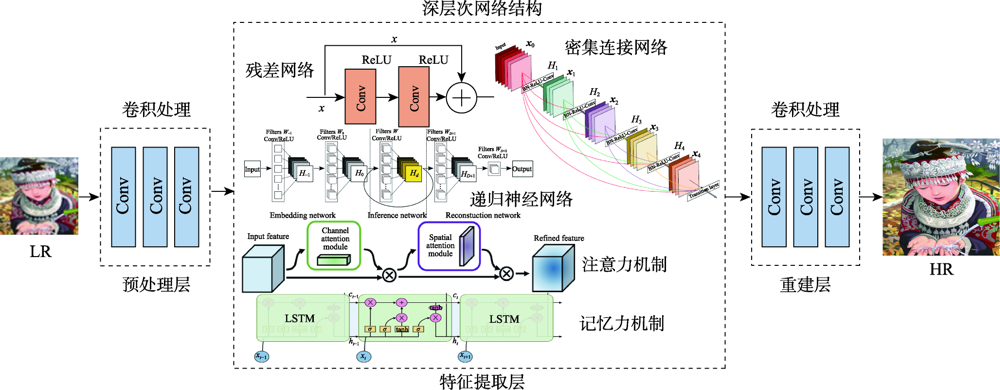
\includegraphics[width=\linewidth]{9.png}
	\caption{深度学习背景下的图像重建网络结构基本图}
	\label{fig:fig9}
\end{figure*}

\begin{table*}[!ht]
\centering
\caption{深度学习背景下的部分网络结构}
\begin{adjustbox}{width=\linewidth}
\begin{tabular}{ccc}
\toprule
	类型 &  作用 &  代表算法 \\ \hline
	 残差学习 &  提高网络收敛速度,学习丰富的复杂特征等 &  VDSR、DRCN、RDN、EDSR等 \\ \hline
	 递归学习 &  缓解梯度爆炸或消失,多路径递归学习等 &  DRCN、DRRN、SRFBN、CDC等 \\ \hline
	 密集连接 &  加强不同层之间的图像传播、利用、融合等 &  SRFBN、SRDenseNet、ESRGAN等 \\ \hline
	 跳跃连接 &  增强层间联系以及特征信息流的传递等 &  DRCN、SRDenseNet、EDSR等 \\ \hline
	 注意力机制 &  标定图像重点与非重点学习重建区域,充分挖掘层内特征信息等 &  RCAN、CBAM、SMSR、CDC、SA-SR-GAN、HAN等 \\ \hline
	 连续记忆机制 &  全局性图像特征融合,连续记忆性传递低频、高频特征信息等 &  RDN、DRRN、SRFBN、SRGAN等 \\ \hline
	 反馈机制 &  共享权重值,确保高级信息与低级信息间的表达与交流等 &  SRFBN、SRGAN、ESRGAN、SRFeat等 \\ \bottomrule
\end{tabular}
\end{adjustbox}
\label{tab:tab2}
\end{table*}

Dong 等人 \cite{DBLP:conf/iccvw/YoonJYLK15}首次将卷积神经网络与超分辨率图像重建技术结合,提出 SRCNN 算法。通过大量卷积 对输入的 LR 图像进行特征提取,不断学习众多图像 的特征表达形式,其重建效果与重建效率远超以往 的图像重建算法,且模型的泛化能力也更强。随后研究者们提出了一 系列不断优化的算法模型,从最早的基于卷积神经网络的 SRCNN(super-resolution convolutional neural net- work)模型,到基于生成对抗网络的 SRGAN(super- resolution generative adversarial network)模型 \cite{DBLP:conf/cvpr/LedigTHCCAATTWS17},再到 基 于 最 新 的 Transformer 的 TTSR(texture trans- former network for SR)模型 \cite{DBLP:conf/cvpr/YangYFLG20},基于深度学习的图像 超分重建技术不断取得新的突破。

\begin{figure*}[!hb]
  \centering
  \begin{minipage}[b]{\linewidth} 
    \subfloat[]{
    \begin{minipage}[b]{0.24\linewidth}
      \centering
      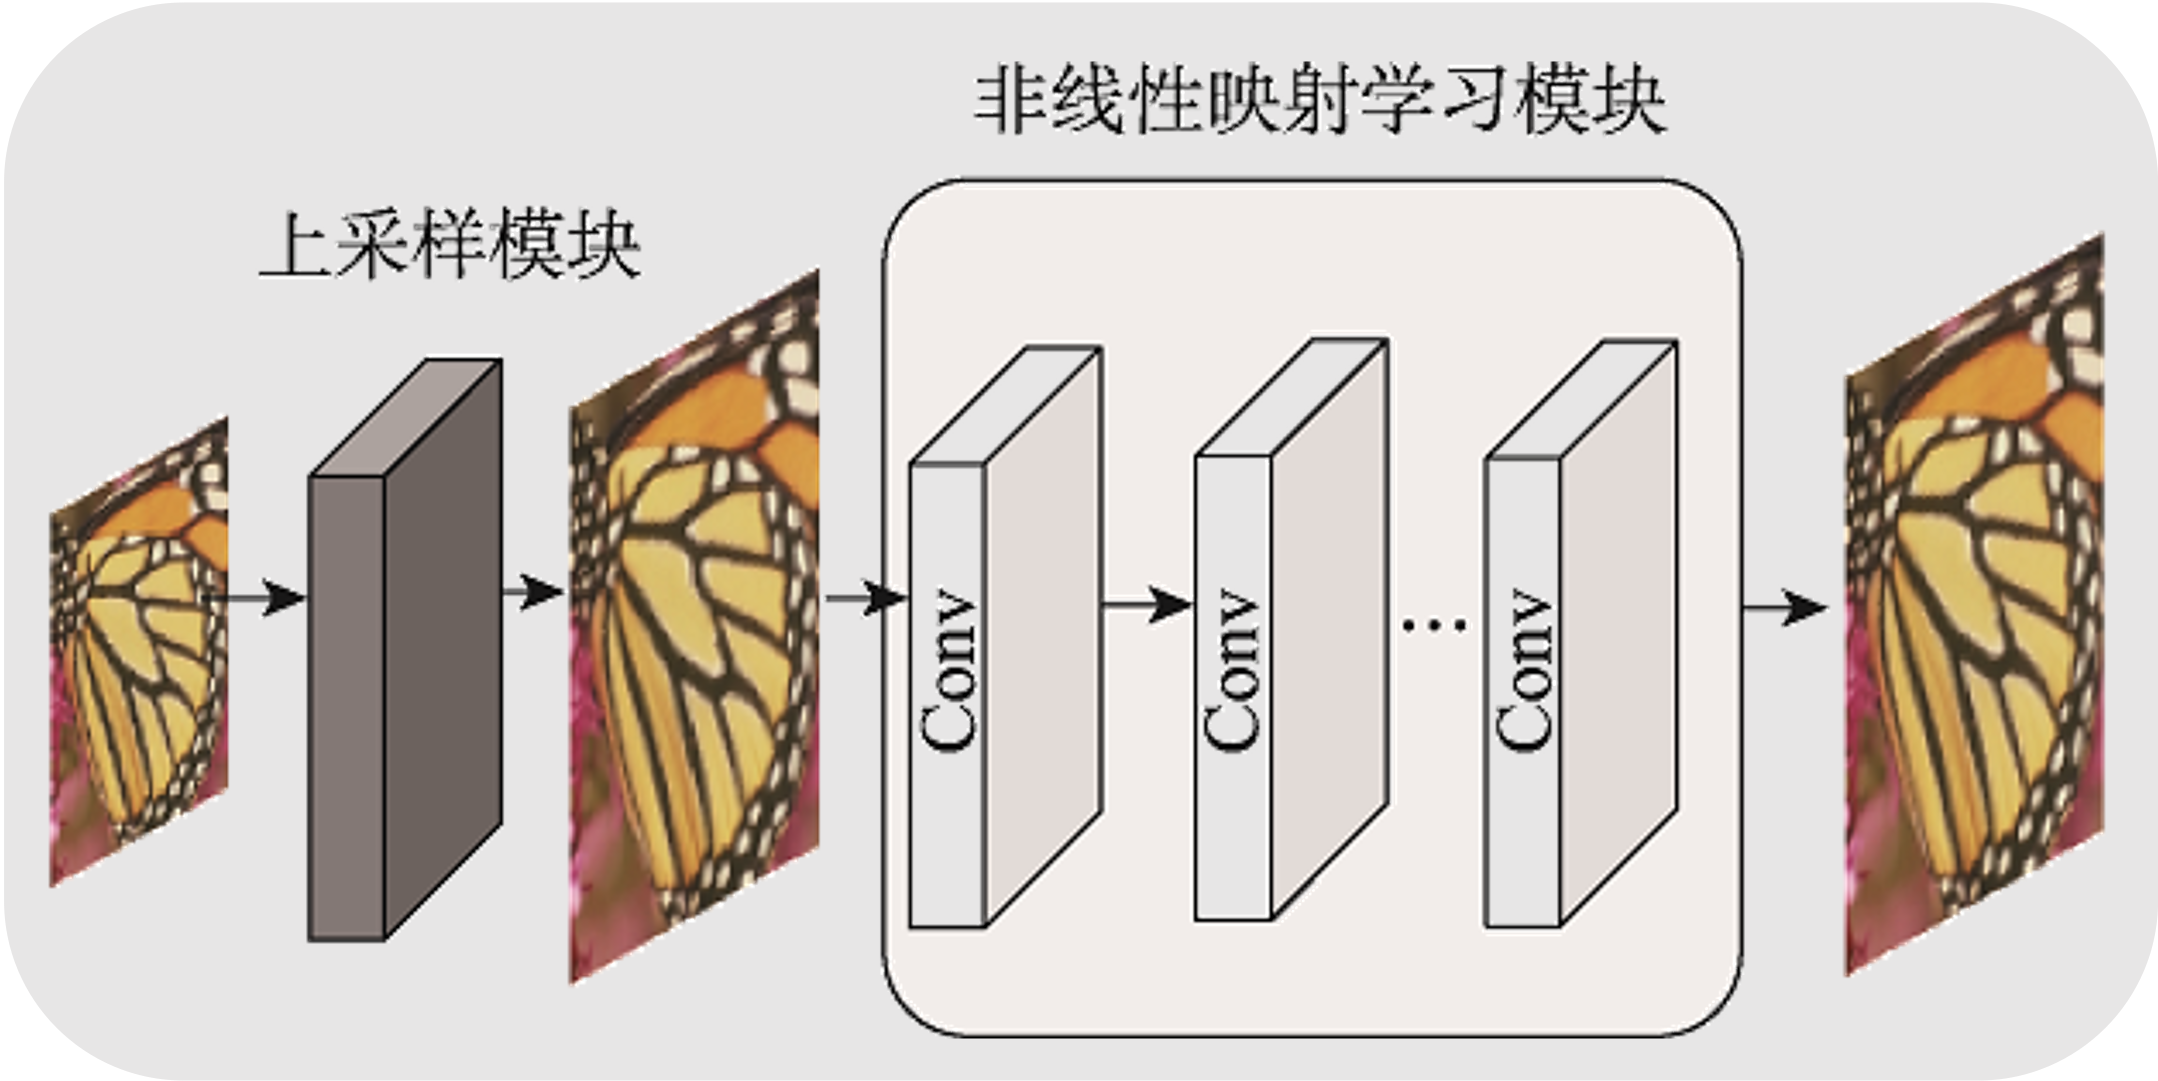
\includegraphics[width=\linewidth]{13-1.png}
     \end{minipage}
  }
   \subfloat[]{
    \begin{minipage}[b]{0.24\linewidth}
      \centering
      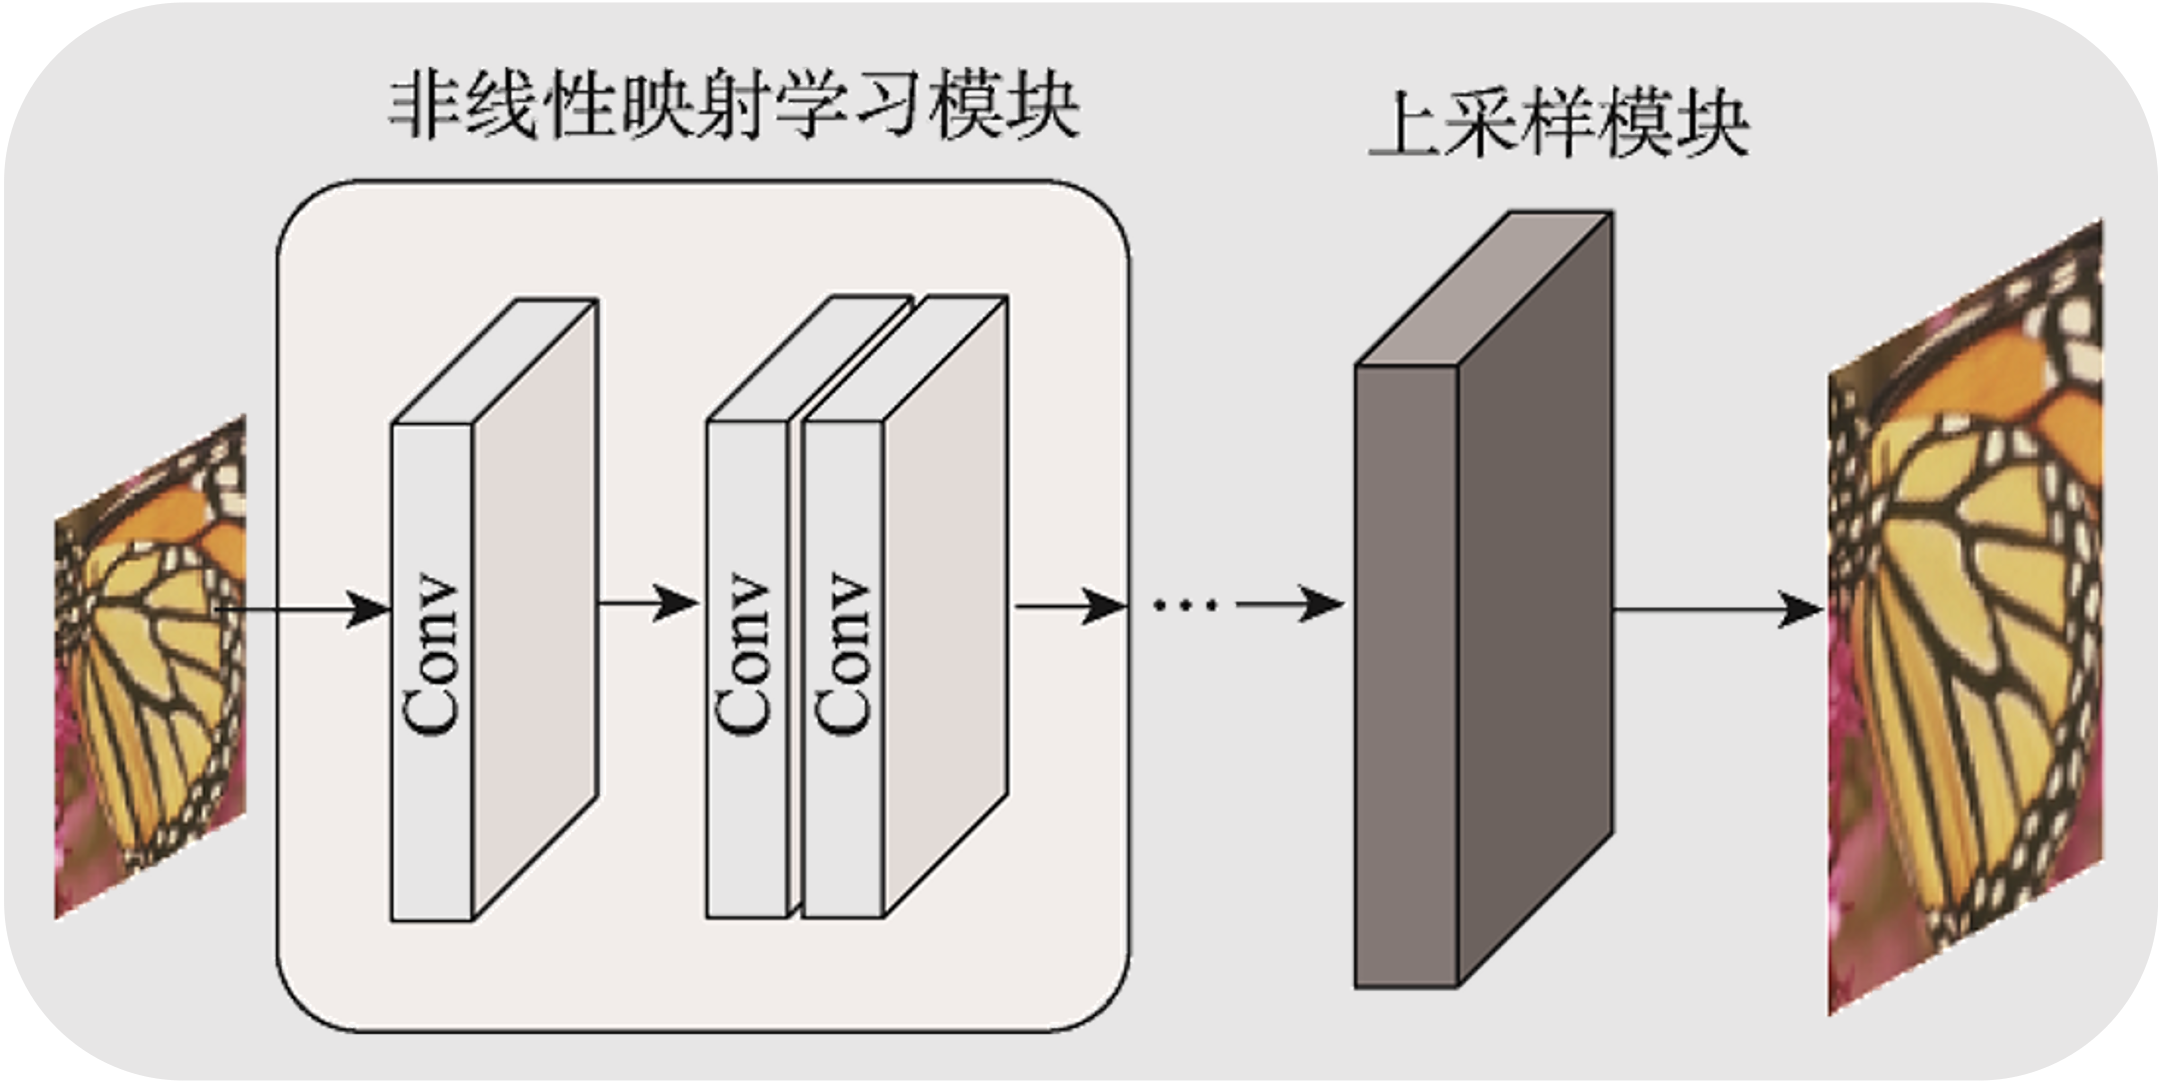
\includegraphics[width=\linewidth]{13-2.png}
     \end{minipage}
  }
  \subfloat[]{
    \begin{minipage}[b]{0.24\linewidth}
      \centering
      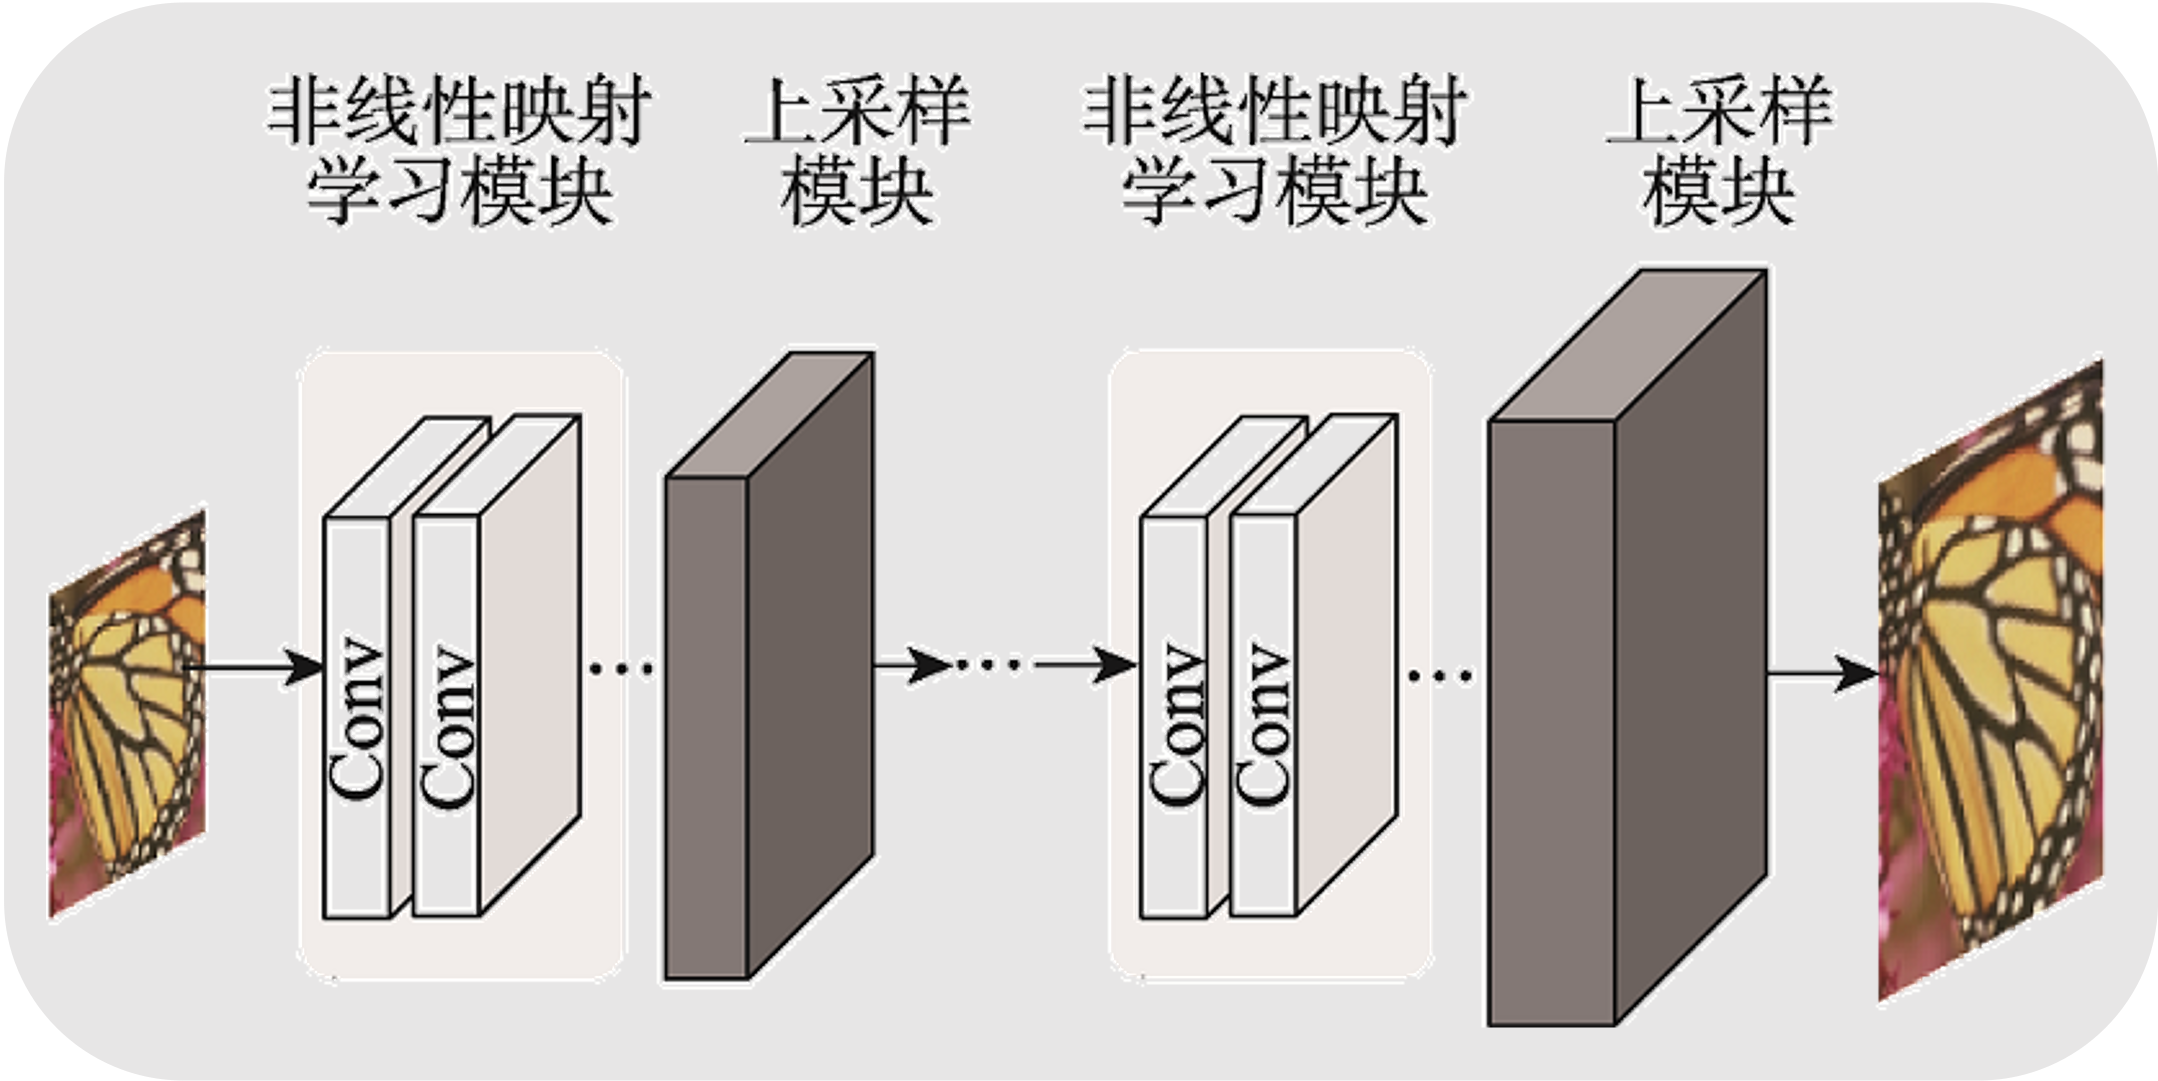
\includegraphics[width=\linewidth]{13-3.png}
     \end{minipage}
  }
   \subfloat[]{
    \begin{minipage}[b]{0.24\linewidth}
      \centering
      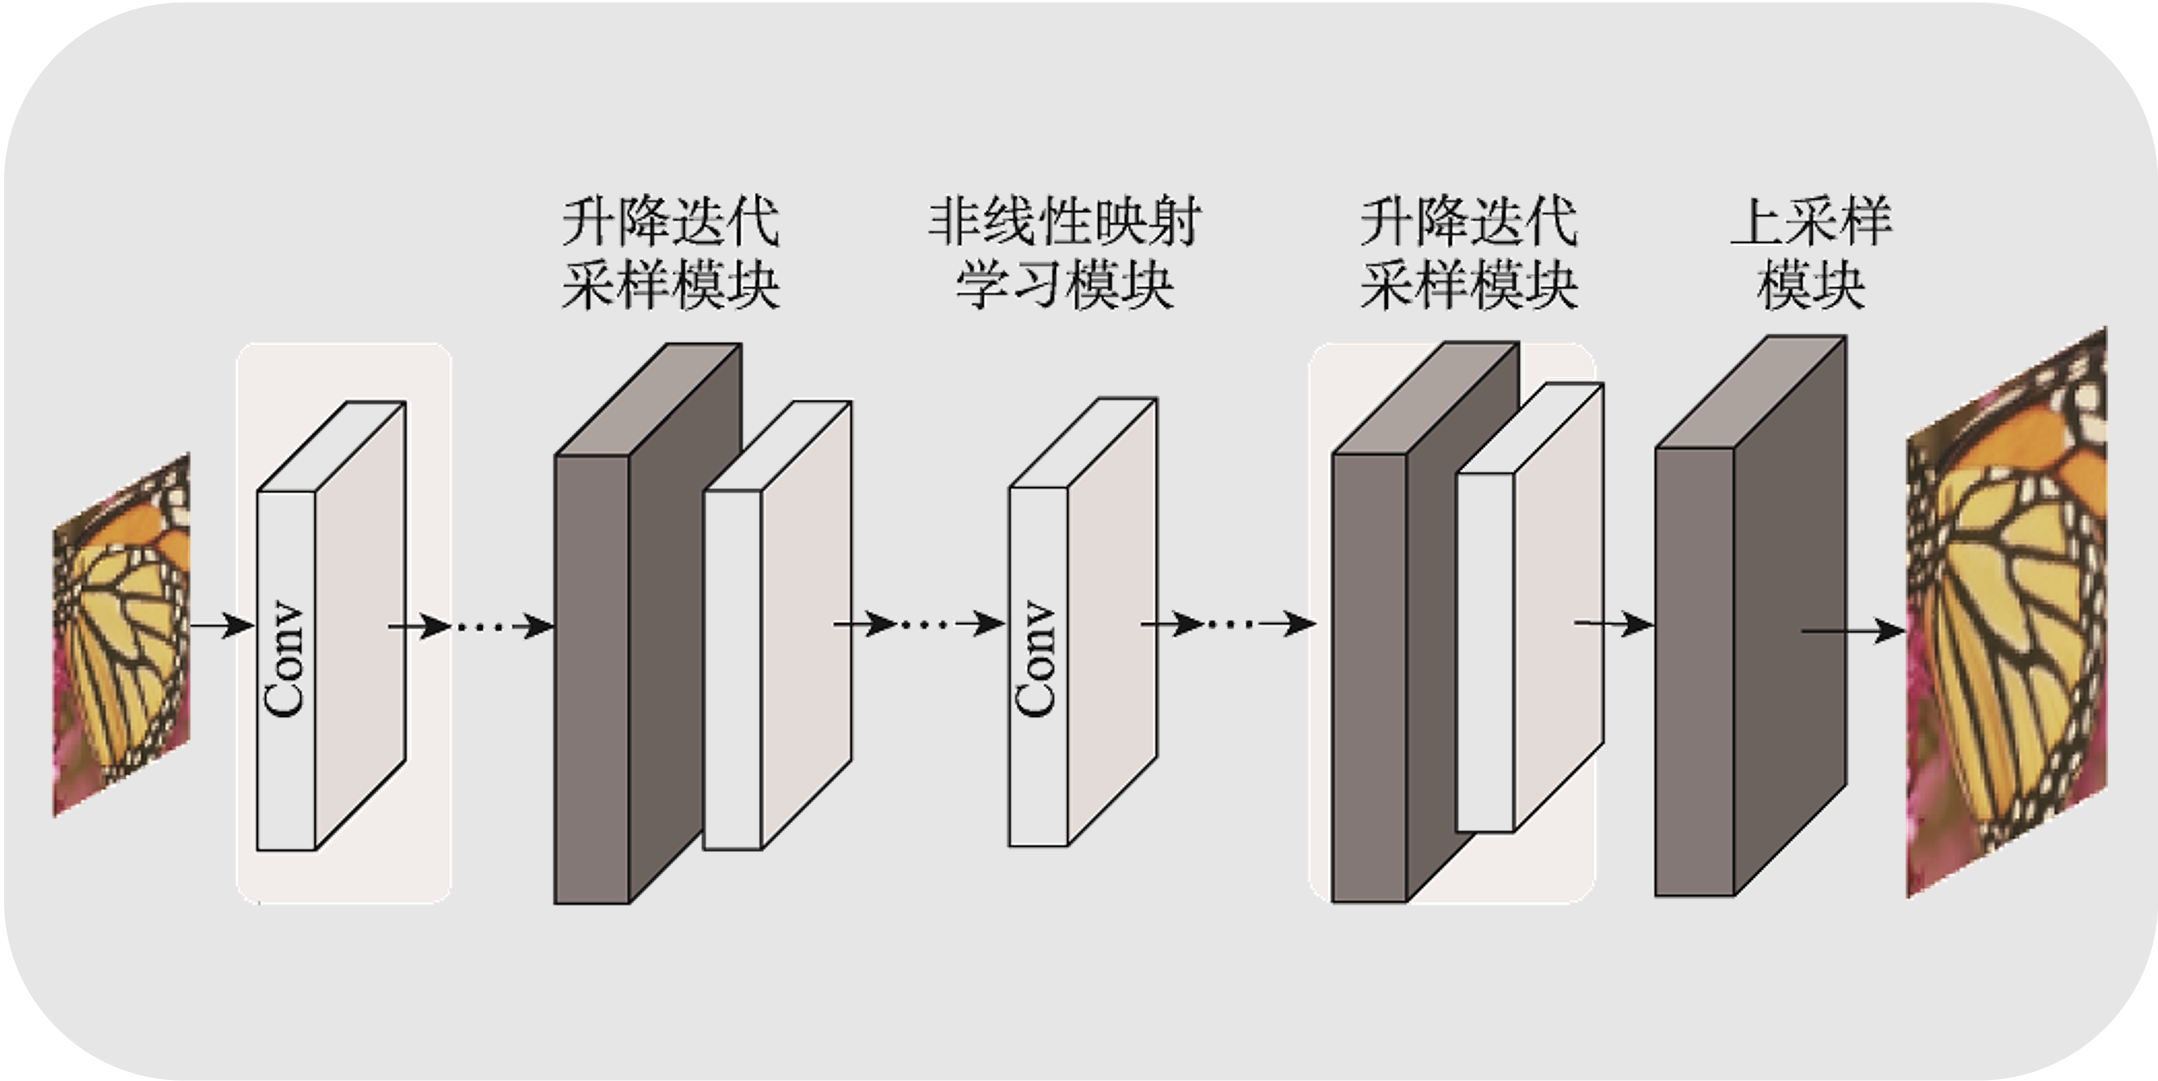
\includegraphics[width=\linewidth]{13-4.png}
     \end{minipage}
  }
    \end{minipage}
  \caption{上采样模块位置不同的超分网络框架:(a) 前端上采样框架;(b) 后端上采样框架;(c) 渐进式上采样框架;(d) 升降采样迭代式框架}
  \label{fig:fig13}
\end{figure*}

SISR 方法的框架由两部分构成,分别是非线性映射学习模块和实现图像放大的上采样模块。非线 性映射学习模块负责完成低分辨率图像到高分辨率 图像的映射,这个过程中利用损失函数来进行引导 和监督学习的进程;上采样模块实现重建图像的放大。两个模块共同协作,最终完成输入图像的超分辨 率重建。根据上采样模块的位置不同,可以将SISR方 法总结为如 \textbf{图 \ref{fig:fig13}} 所示四种超分框架:

\begin{itemize}
	\item \textbf{前端上采样超分框架}可以避免在低维空间上 进行低维到高维的映射学习,降低了学习难度,是一 种简单易行的方法。但是同时噪声和模糊等也被增 强,并且在高维空间进行卷积运算将会增加模型计 算量,消耗更多的计算资源。
	\item \textbf{后端上采样超分框架}针对前端 上采样超分框架存在的问题,提高计算资源利用效 率,研究者提出了后端上采样超分框架,将上采样模 块放置在网络后面部分。该框架下的大部分卷积计算在低维空间进行,最后再利用端到端可学习的上 采样层,如转置卷积和亚像素卷积,进行上采样 放大。这样的好处是进一步释放了卷积的计算能力, 降低模型复杂度。
	\item \textbf{渐进式上采样超分框架}中,图像放大是逐级进行的,中途生成的图像继续输入后续模块,直到达到 目标分辨率。常用方法是采用卷积级联或者 Laplace 金字塔的方式,再结合多级监督等学习策略,就能完 成大的超分倍增系数下的超分重建任务。
	\item \textbf{升降采样迭代式超分框架}借 鉴了反向投影的思想,交替使用上、下采样,结合得到的所有特征图来完成 低分辨率图像的重建。这种方法通过反复进行 LR- HR 的映射学习,能充分学习出两者之间的映射关 系。
\end{itemize}

\begin{figure}[!t]
	\centering
	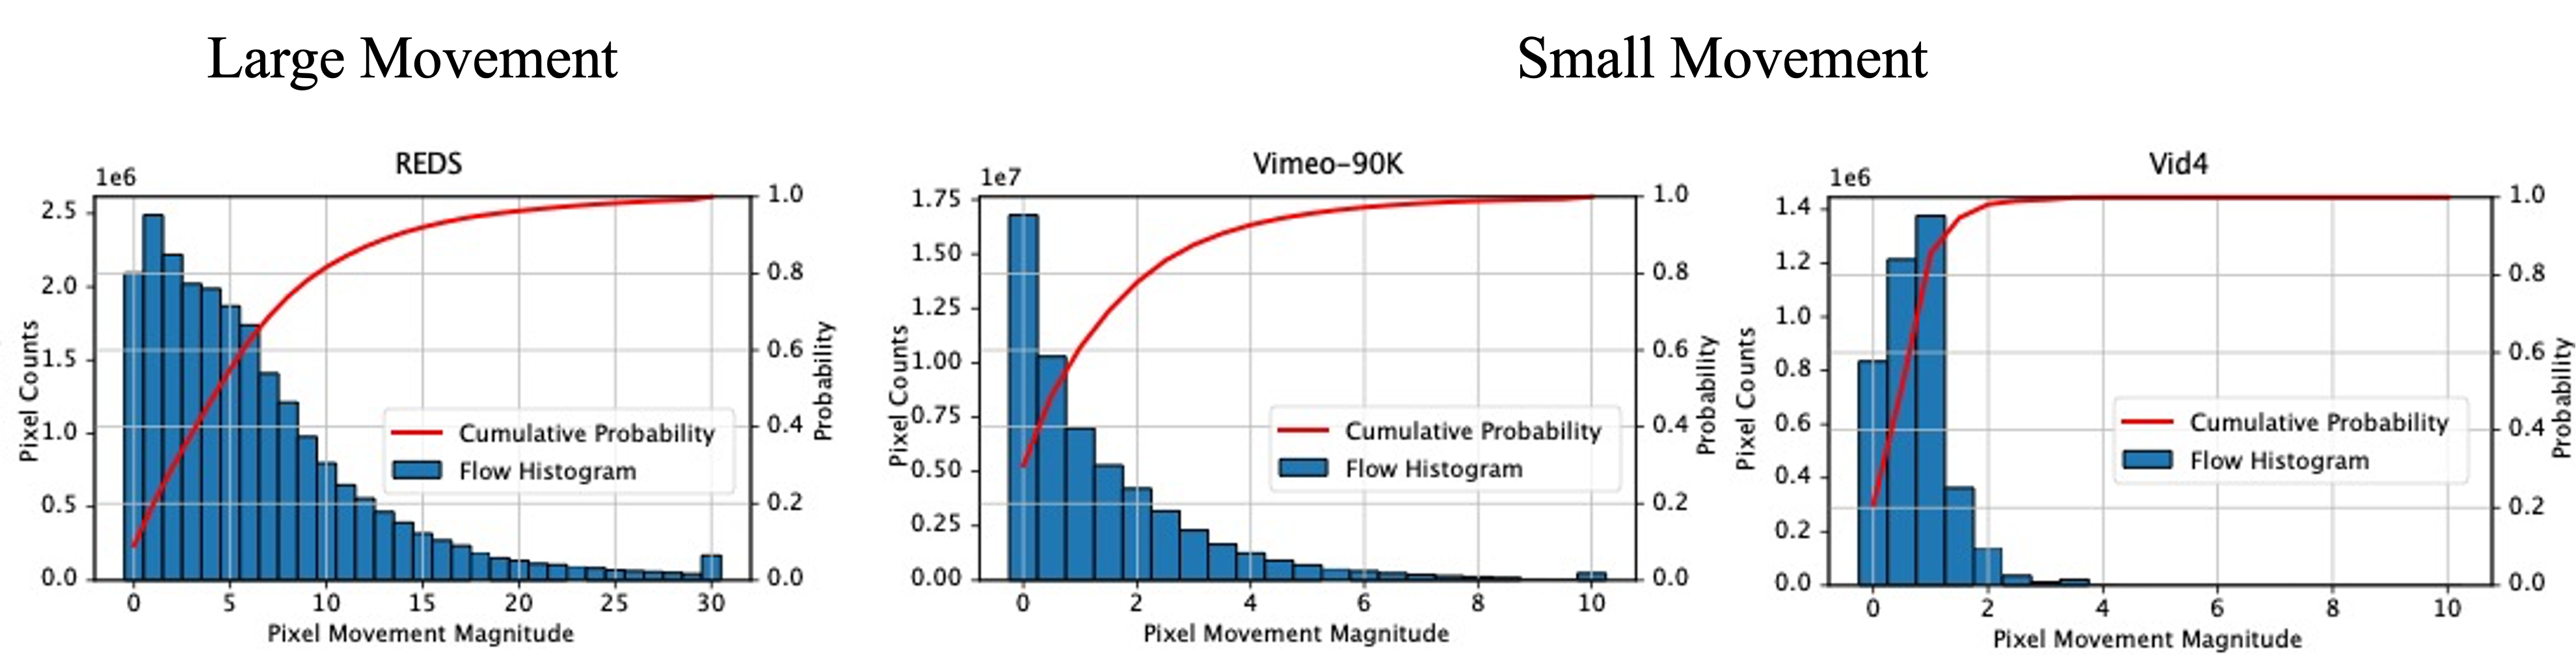
\includegraphics[width=\linewidth]{10}
	\caption{用于图像超分辨率重建网络解释的局部归因图(LAM Attribution, LAM)方法的可视化结果。LAM 图表示输入 LR 图像中每个像素的重要性}
	\label{fig:fig10}
\end{figure}

传统的基于卷积神经网络的图像超分辨率重建方法,为了建立 LR 图像和 HR 图像的映射关系并能恢复图像更加精细的细节,大多从模型的骨干网络(如 VGG、ResNet),上采样方法(如反卷积、亚像素层),多尺度策略(如特征金字塔、密集连接),注意力机制(如通道注意力和空间注意力)等来充分地利用低分辨率图像的先验信息,重建出缺失的高频信息。除了对网络架构和模块设计的研究, Dong 等 \cite{DBLP:conf/cvpr/GuD21}从超分网络可解释性的角度对图像重建进行研究,利用局部归因局部归因图的方法对超分结果进行归因分析。如 \textbf{图 \ref{fig:fig10}} 是一张 LR 图通过不同的模型超分成一张 SR 图的结果。HR 图上有一个红色的框,LAM Attribution 就代表了三个不同的超分模型输入的 LR 图像中每个像素对红色的框 SR 结果的重要性。对 HR 图像中间红框处的超分结果进行归因分析,右边图像上标红的像素即为对该超分结果``贡献比较大''的像素。LAM 结果表明,FSRCNN 仅利用非常有限的信息,EDSR 增加了信息利用的范围,但仍然无法重建精确的纹理,而非局部网络 RNAN 可以利用更大范围的信息来获得更好的超分结果。

\begin{figure*}[!htbp]
	\centering
	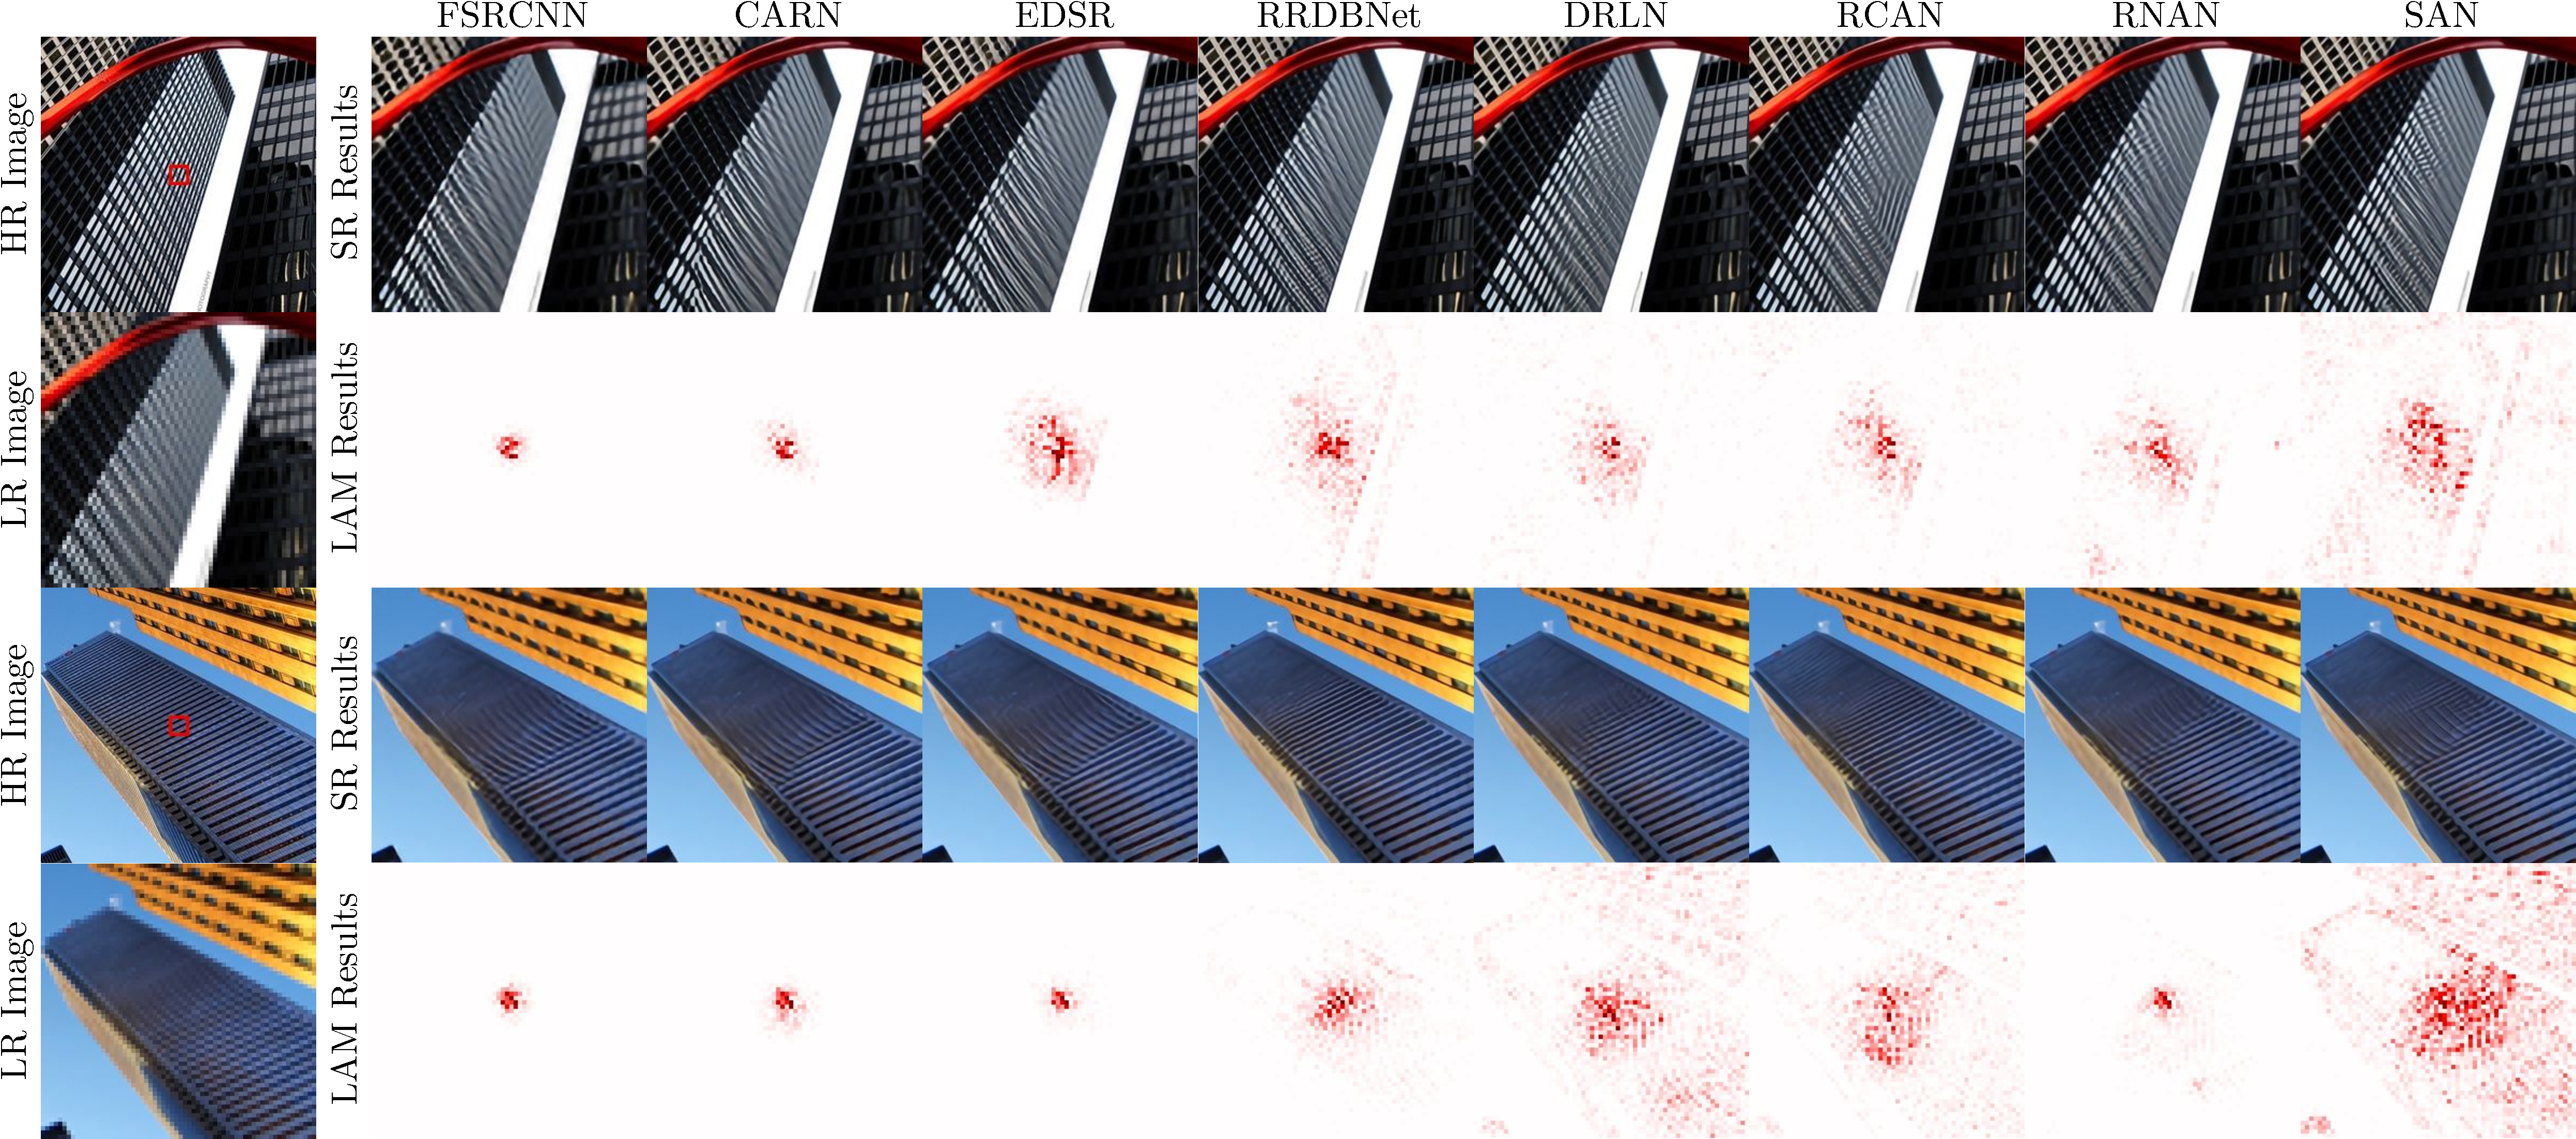
\includegraphics[width=\linewidth]{11}
	\caption{LAM 实验结果}
	\label{fig:fig11}
\end{figure*}

不同 SR 模型的 LAM 结果如 \textbf{图 \ref{fig:fig11}} 所示。有以下的观察:

\begin{enumerate}
	\item 早期的网络 FSRCNN 和浅层网络 CARN 的归因图有效区域相对较小,意味着这些模型只能基于有限的周围像素进行超分。
	\item 深度残差网络,即 EDSR,RRDBNet,RCAN 和 DRLN,具有更深的架构和更大的归因图有效区域。这些网络对 LR 图像中具有相似图案的更大范围的像素感兴趣,例如,摩天大楼上出现的规则条纹。尽管这些区域中的纹理在 LR 图像中严重混叠,这可能误导 SR 过程,但是一些网络仍然重建精确的纹理,并且根据 LAM 结果,它们注意到更大范围的未混叠区域。
	\item 对于有 non-local 和 channel-wise attention 模块的超分模型,它们会利用更长距离的信息来协助 SR 的过程。代表性模型包括 RNAN,RNAN 和 SAN。
\end{enumerate}

受 Transformer 在诸多计算机视觉任务上取得优异表现的驱动,越来越多的研究也将其引入到图像超分辨率重建任务中,并一度刷新图像超分辨率重建的性能。显然,这得益于 Transformer 对远程依赖建模的能力,使得他相比较于卷积神经网络模型可以看到更多的像素。但 Dong 等人 \cite{DBLP:journals/corr/abs-2205-04437}利用局部归因图研究发现对于 CNN-based methods 例如 RCAN,EDSR 这一想法是正确的。然而对于 Transformer-based method SwinIR 来讲,LAM 的结果并没有表明 SwinIR 比 RCAN 利用的信息多。说明 SwinIR 比 CNN 有更强的映射能力,能利用更少的信息获得更好的效果。其次,SwinIR 在 exploit input pixels 仍有提升空间。基于此,他们设计了 Hybrid Attention Transformer 来结合 channel attention 和 self-attention 两种方案,以利用前者对全局信息的利用能力和后者强大的表示能力。 此外,为了更好地聚合跨窗口信息,引入了一个重叠的交叉注意模块。实验结果如 \textbf{表 \ref{quantitative results}} 所示,可以看到, Transformer-based method 几乎已经成为图像超分辨率重建任务的主流研究框架。

如 \textbf{图 \ref{fig:fig12}} 所示的热图展示了不同 SR 网络的关注区域,所有的 SR 网络都关注红色的区域,不同 SR 模型关注区域的不同体现在蓝色区域上。 如何提取和利用蓝色区域的信息是一个 SR 网络区别于其他网络的关键因素。在图6的第6、第7和第8个例子中,SR 网络的注意力沿着纹理延伸的方向分布;在第9个例子中,SR 网络注意到目标补丁周围形状相似的窗口。

\begin{figure*}[!htbp]
	\centering
	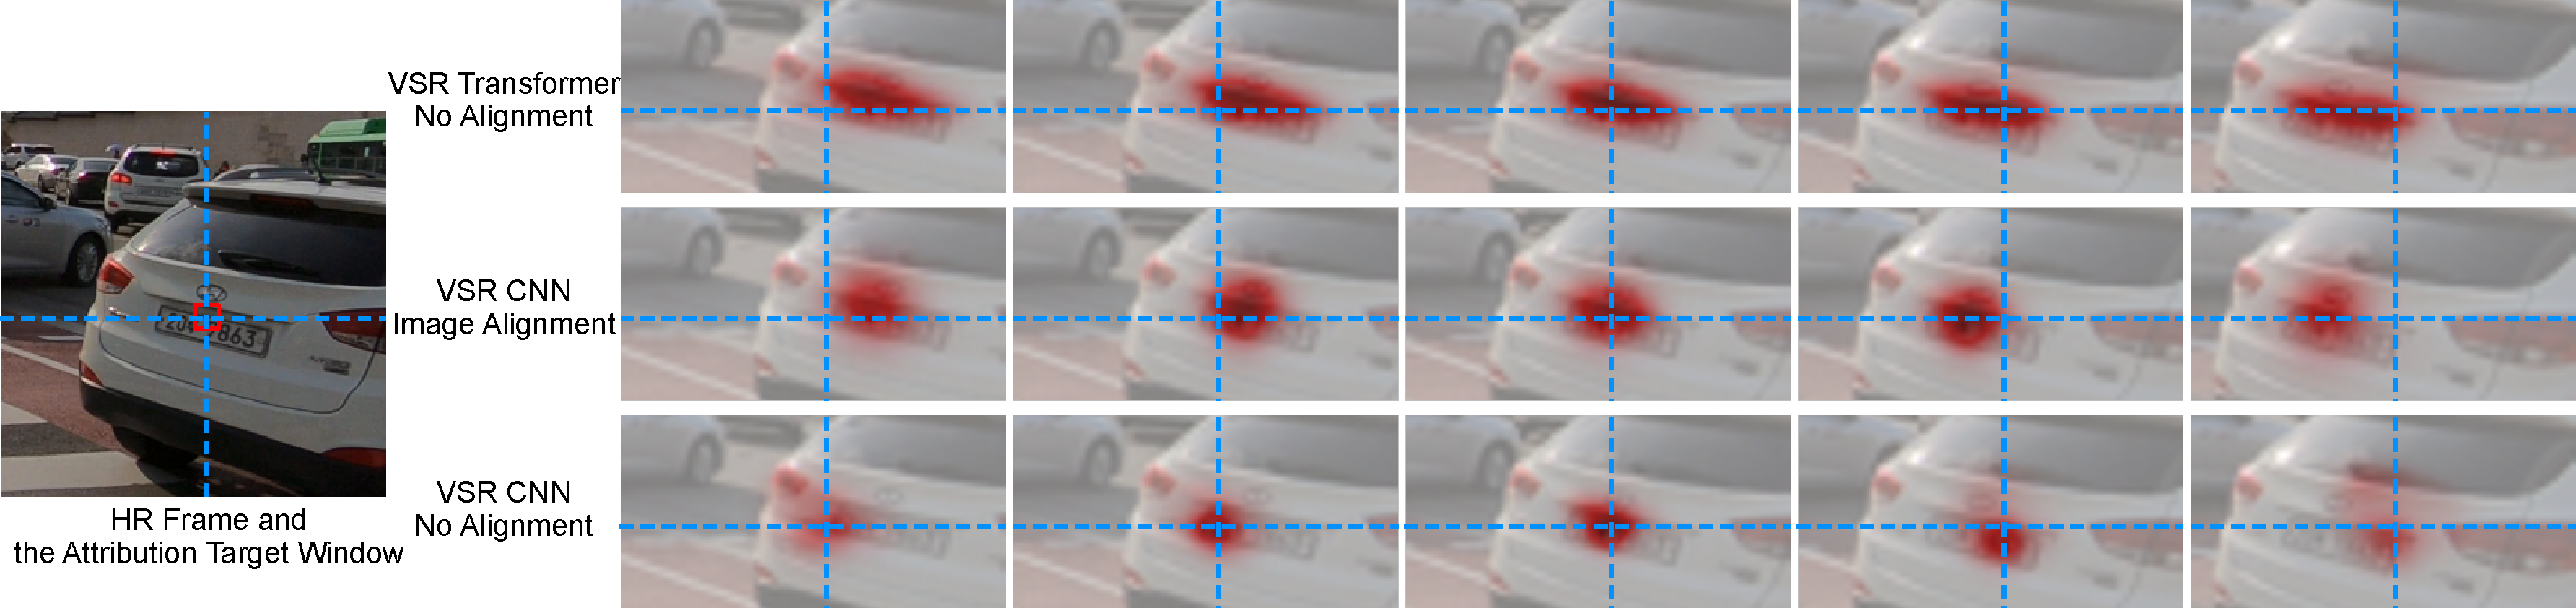
\includegraphics[width=\linewidth]{12}
	\caption{热图展示了不同 SR 网络的关注区域,所有 SR 网络都关注红色的区域,不同 SR 模型关注区域的不同体现在蓝色区域}
	\label{fig:fig12}
\end{figure*}


\begin{table*}[!htbp]
\scriptsize
\center
\begin{center}
\caption{在基准数据集上与 SOTA 的方法进行定量比较。前三的方法用 \textcolor{red}{红色}, \textcolor{blue}{蓝色} 和~  {\color[HTML]{00BF01} 绿色} 标注。 ``$\dagger$'' 表示该方法在 ImageNet 上进行预训练}
\label{quantitative results}
\begin{adjustbox}{width=\linewidth}
\renewcommand{\arraystretch}{1.3}
% \linespread{1.3}
% \vspace{2mm}
%\resizebox{\textwidth}{70mm}{
\begin{tabular}{|l|c|c|c|c|c|c|c|c|c|c|c|c|}
\hline
\multirow{2}{*}{Method} & \multirow{2}{*}{Scale} & \multirow{2}{*}{\makecell{Training\\Dataset}} &
\multicolumn{2}{c|}{Set5~\cite{DBLP:conf/bmvc/BevilacquaRGA12}} &  \multicolumn{2}{c|}{Set14~\cite{DBLP:conf/cas/ZeydeEP10}} &  \multicolumn{2}{c|}{BSD100~\cite{DBLP:conf/iccv/MartinFTM01}} &  \multicolumn{2}{c|}{Urban100~\cite{DBLP:conf/cvpr/HuangSA15}} &  \multicolumn{2}{c|}{Manga109~\cite{DBLP:journals/mta/MatsuiIAFOYA17}}  
\\ 
%\hline
\cline{4-13}
&  &  & PSNR & SSIM & PSNR & SSIM & PSNR & SSIM & PSNR & SSIM & PSNR & SSIM 
\\ 
\hline
\hline
EDSR~\cite{DBLP:conf/cvpr/LimSKNL17} & $\times$2 & DIV2K %
& 38.11
& 0.9602
& 33.92
& 0.9195
& 32.32
& 0.9013
& 32.93
& 0.9351
& 39.10
& 0.9773
\\
RCAN~\cite{DBLP:journals/corr/abs-2201-11279} & $\times$2 & DIV2K %
& 38.27
& 0.9614
& 34.12
& 0.9216
& 32.41
& 0.9027
& 33.34
& 0.9384
& 39.44
& 0.9786
\\  
SAN~\cite{DBLP:conf/cvpr/DaiCZXZ19} & $\times$2 & DIV2K %
& {38.31}
& {0.9620}
& {34.07}
& {0.9213}
& {32.42}
& {0.9028}
& {33.10}
& {0.9370}
& {39.32}
& {0.9792}\\
IGNN~\cite{zhou2020cross} & $\times$2 & DIV2K %
& {38.24}
& {0.9613}
& {34.07}
& {0.9217}
& {32.41}
& {0.9025}
& {33.23}
& {0.9383}
& {39.35}
& {0.9786}
\\
HAN~\cite{niu2020single} & $\times$2 & DIV2K %
& {38.27}
& {0.9614}
& {34.16}
& {0.9217}
& {32.41}
& {0.9027}
& {33.35}
& {0.9385}
& {39.46}
& {0.9785}              
\\
NLSN~\cite{mei2021image} & $\times$2 & DIV2K %
& 38.34 
& 0.9618 
& 34.08 
& 0.9231
& 32.43 
& 0.9027 
& 33.42
& 0.9394
& 39.59
& 0.9789
\\
RCAN-it~\cite{DBLP:journals/corr/abs-2201-11279} & $\times$2 & DF2K %
& 38.37
& 0.9620
& 34.49
& 0.9250
& 32.48
& 0.9034
& 33.62
& 0.9410
& 39.88
& 0.9799
\\
SwinIR~\cite{DBLP:conf/iccvw/LiangCSZGT21} & $\times$2 & DF2K %
& 38.42
& 0.9623
& 34.46
& 0.9250
& 32.53
& 0.9041
& 33.81
& 0.9427
& 39.92
& 0.9797
\\
EDT~\cite{DBLP:journals/corr/abs-2112-10175} & $\times$2 & DF2K %
& 38.45
& 0.9624
& 34.57
& 0.9258
& 32.52
& 0.9041
& 33.80
& 0.9425
& 39.93
& 0.9800
\\
\textbf{HAT} (ours) & $\times$2 & DF2K %
& {\color[HTML]{00BF01} 38.63}
& {0.9630}
& {\color[HTML]{00BF01} 34.86}
& {\color[HTML]{00BF01} 0.9274}
& {\color[HTML]{00BF01} 32.62}
& {\color[HTML]{00BF01} 0.9053}
& {\color[HTML]{00BF01} 34.45}
& {\color[HTML]{00BF01} 0.9466}
& {40.26}
& {0.9809}
\\
\hdashline
IPT$^\dagger$~\cite{DBLP:conf/cvpr/Chen000DLMX0021} & $\times$2 & ImageNet %
& {38.37}
& {-}
& {34.43}
& {-}
& {32.48}
& {-}
& {33.76}
& {-}
& {-}
& {-}
\\
EDT$^\dagger$~\cite{DBLP:journals/corr/abs-2112-10175} & $\times$2 & DF2K %
& {\color[HTML]{00BF01} 38.63}
& {\color[HTML]{00BF01} 0.9632}
& 34.80
& 0.9273
& {\color[HTML]{00BF01} 32.62}
& {0.9052}
& 34.27
& 0.9456
& {\color[HTML]{00BF01} 40.37}
& {\color[HTML]{00BF01} 0.9811}
\\
\textbf{HAT}$^\dagger$ (ours) & $\times$2 & DF2K %
& \textcolor{blue}{38.73}
& \textcolor{blue}{0.9637}
& \textcolor{blue}{35.13}
& \textcolor{blue}{0.9282}
& \textcolor{blue}{32.69}
& \textcolor{blue}{0.9060}
& \textcolor{blue}{34.81}
& \textcolor{blue}{0.9489}
& \textcolor{blue}{40.71}
& \textcolor{blue}{0.9819}
\\
\textbf{HAT-L}$^\dagger$ (ours) & $\times$2 & DF2K %
& \textcolor{red}{38.91}
& \textcolor{red}{0.9646}
& \textcolor{red}{35.29}
& \textcolor{red}{0.9293}
& \textcolor{red}{32.74}
& \textcolor{red}{0.9066}
& \textcolor{red}{35.09}
& \textcolor{red}{0.9505}
& \textcolor{red}{41.01}
& \textcolor{red}{0.9831}
\\
\hline
\hline
EDSR~\cite{DBLP:conf/cvpr/LimSKNL17} & $\times$3 & DIV2K %
& 34.65
& 0.9280
& 30.52
& 0.8462
& 29.25
& 0.8093
& 28.80
& 0.8653
& 34.17
& 0.9476
\\
RCAN~\cite{DBLP:journals/corr/abs-2201-11279} & $\times$3 & DIV2K %
& 34.74
& 0.9299
& 30.65
& 0.8482
& 29.32
& 0.8111
& 29.09
& 0.8702
& 34.44
& 0.9499
\\
SAN~\cite{DBLP:conf/cvpr/DaiCZXZ19} & $\times$3 & DIV2K %
& {34.75}
& {0.9300}
& {30.59}
& {0.8476}
& {29.33}
& {0.8112}
& {28.93}
& {0.8671}
& {34.30}
& {0.9494}
\\
IGNN~\cite{zhou2020cross} & $\times$3 & DIV2K %
& {34.72}
& {0.9298}
& {30.66}
& {0.8484}
& {29.31}
& {0.8105}
& {29.03}
& {0.8696}
& {34.39}
& {0.9496}
\\
HAN~\cite{niu2020single}  & $\times$3 & DIV2K %
& {34.75}
& {0.9299}
& {30.67}
& {0.8483}
& {29.32}
& {0.8110}
& {29.10}
& {0.8705}
& {34.48}
& {0.9500}
\\
NLSN~\cite{mei2021image} & $\times$3 & DIV2K %
& 34.85 
& 0.9306 
& 30.70 
& 0.8485 
& 29.34 
& 0.8117 
& {29.25}
& {0.8726}
& 34.57 
& 0.9508  
\\
RCAN-it~\cite{DBLP:journals/corr/abs-2201-11279} & $\times$3 & DF2K %
& {34.86}
& {0.9308}
& {30.76}
& {0.8505}
& {29.39}
& {0.8125}
& {29.38}
& {0.8755}
& {34.92}
& {0.9520}
\\
SwinIR~\cite{DBLP:conf/iccvw/LiangCSZGT21} & $\times$3 & DF2K %
& 34.97
& 0.9318
& 30.93
& 0.8534
& 29.46
& 0.8145
& 29.75
& 0.8826
& 35.12
& 0.9537
\\
EDT~\cite{DBLP:journals/corr/abs-2112-10175} & $\times$3 & DF2K %
& 34.97
& 0.9316
& 30.89
& 0.8527
& 29.44
& 0.8142
& 29.72
& 0.8814
& 35.13
& 0.9534
\\
\textbf{HAT} (ours) & $\times$3 & DF2K %
& {35.06}
& {\color[HTML]{00BF01} 0.9329}
& {31.08}
& {\color[HTML]{00BF01} 0.8555}
& {\color[HTML]{00BF01} 29.54}
& {\color[HTML]{00BF01} 0.8167}
& {\color[HTML]{00BF01} 30.23}
& {\color[HTML]{00BF01} 0.8896}
& {\color[HTML]{00BF01} 35.53}
& {\color[HTML]{00BF01} 0.9552}
\\
\hdashline
IPT$^\dagger$~\cite{DBLP:conf/cvpr/Chen000DLMX0021} & $\times$3 & ImageNet %
& {34.81}
& {-}
& {30.85}
& {-}
& {29.38}
& {-}
& {29.49}
& {-}
& {-}
& {-}
\\
EDT$^\dagger$~\cite{DBLP:journals/corr/abs-2112-10175} & $\times$3 & DF2K %
& {\color[HTML]{00BF01} 35.13}
& 0.9328
& {\color[HTML]{00BF01} 31.09}
& 0.8553
& {29.53}
& {0.8165}
& 30.07
& 0.8863
& 35.47
& 0.9550
\\
\textbf{HAT}$^\dagger$ (ours) & $\times$3 & DF2K %
& \textcolor{blue}{35.16}
& \textcolor{blue}{0.9335}
& \textcolor{blue}{31.33}
& \textcolor{blue}{0.8576}
& \textcolor{blue}{29.59}
& \textcolor{blue}{0.8177}
& \textcolor{blue}{30.70}
& \textcolor{blue}{0.8949}
& \textcolor{blue}{35.84}
& \textcolor{blue}{0.9567}
\\
\textbf{HAT-L}$^\dagger$ (ours) & $\times$3 & DF2K %
& \textcolor{red}{35.28}
& \textcolor{red}{0.9345}
& \textcolor{red}{31.47}
& \textcolor{red}{0.8584}
& \textcolor{red}{29.63}
& \textcolor{red}{0.8191}
& \textcolor{red}{30.92}
& \textcolor{red}{0.8981}
& \textcolor{red}{36.02}
& \textcolor{red}{0.9576}
\\
\hline
\hline
EDSR~\cite{DBLP:conf/cvpr/LimSKNL17} & $\times$4 & DIV2K %
& 32.46
& 0.8968
& 28.80
& 0.7876
& 27.71
& 0.7420
& 26.64
& 0.8033
& 31.02
& 0.9148
\\
RCAN~\cite{DBLP:journals/corr/abs-2201-11279} & $\times$4 & DIV2K %
& 32.63
& 0.9002
& 28.87
& 0.7889
& 27.77
& 0.7436
& 26.82
& 0.8087
& 31.22
& 0.9173
\\
SAN~\cite{DBLP:conf/cvpr/DaiCZXZ19} & $\times$4 & DIV2K %
& {32.64}
& {0.9003}
& {28.92}
& {0.7888}
& {27.78}
& {0.7436}
& {26.79}
& {0.8068}
& {31.18}
& {0.9169}
\\
IGNN~\cite{zhou2020cross} & $\times$4 & DIV2K %
& {32.57}
& {0.8998}
& {28.85}
& {0.7891}
& {27.77}
& {0.7434}
& {26.84}
& {0.8090}
& {31.28}
& {0.9182}
\\
HAN~\cite{niu2020single} & $\times$4 & DIV2K %
& {32.64}
& {0.9002}
& {28.90}
& {0.7890}
& {27.80}
& {0.7442}
& {26.85}
& {0.8094}
& {31.42}
& {0.9177}
\\
NLSN~\cite{mei2021image} & $\times$4 & DIV2K %
& 32.59 
& 0.9000 
& 28.87 
& 0.7891 
& 27.78 
& 0.7444 
& {26.96}
& {0.8109}
& 31.27 
& 0.9184
\\
RRDB~\cite{DBLP:conf/iccvw/WangXDS21} & $\times$4 & DF2K %
& {32.73}
& {0.9011 }
& {28.99}
& {0.7917}
& {27.85}
& {0.7455}
& {27.03}
& {0.8153}
& {31.66}
& {0.9196}
\\
RCAN-it~\cite{DBLP:journals/corr/abs-2201-11279} & $\times$4 & DF2K %
& 32.69
& 0.9007
& 28.99
& 0.7922
& 27.87
& 0.7459
& 27.16
& 0.8168
& 31.78
& 0.9217
\\
SwinIR~\cite{DBLP:conf/iccvw/LiangCSZGT21} & $\times$4 & DF2K %
& 32.92
& 0.9044
& 29.09
& 0.7950
& 27.92
& 0.7489
& 27.45
& 0.8254
& 32.03
& 0.9260
\\
EDT~\cite{DBLP:journals/corr/abs-2112-10175} & $\times$4 & DF2K %
& 32.82
& 0.9031
& 29.09
& 0.7939
& 27.91
& 0.7483
& 27.46
& 0.8246
& 32.05
& 0.9254
\\
\textbf{HAT} (ours) & $\times$4 & DF2K %
& {33.04}
& {\color[HTML]{00BF01} 0.9056}
& {\color[HTML]{00BF01} 29.23}
& {\color[HTML]{00BF01} 0.7973}
& {\color[HTML]{00BF01} 28.00}
& {\color[HTML]{00BF01} 0.7517}
& {\color[HTML]{00BF01} 27.97}
& {\color[HTML]{00BF01} 0.8368}
& {\color[HTML]{00BF01} 32.48}
& {\color[HTML]{00BF01} 0.9292}
\\
\hdashline
IPT$^\dagger$~\cite{DBLP:conf/cvpr/Chen000DLMX0021} & $\times$4 & ImageNet %
& {32.64}
& {-}
& {29.01}
& {-}
& {27.82}
& {-}
& {27.26}
& {-}
& {-}
& {-}
\\
EDT$^\dagger$~\cite{DBLP:journals/corr/abs-2112-10175} & $\times$4 & DF2K %
& {\color[HTML]{00BF01} 33.06}
& {0.9055}
& {\color[HTML]{00BF01} 29.23}
& {0.7971}
& {27.99}
& 0.7510
& 27.75
& 0.8317
& 32.39
& 0.9283
\\
\textbf{HAT}$^\dagger$ (ours) & $\times$4 & DF2K %
& \textcolor{blue}{33.18}
& \textcolor{blue}{0.9073}
& \textcolor{blue}{29.38}
& \textcolor{blue}{0.8001}
& \textcolor{blue}{28.05}
& \textcolor{blue}{0.7534}
& \textcolor{blue}{28.37}
& \textcolor{blue}{0.8447}
& \textcolor{blue}{32.87}
& \textcolor{blue}{0.9319}
\\
\textbf{HAT-L}$^\dagger$ (ours) & $\times$4 & DF2K %
& \textcolor{red}{33.30}
& \textcolor{red}{0.9083}
& \textcolor{red}{29.47}
& \textcolor{red}{0.8015}
& \textcolor{red}{28.09}
& \textcolor{red}{0.7551}
& \textcolor{red}{28.60}
& \textcolor{red}{0.8498}
& \textcolor{red}{33.09}
& \textcolor{red}{0.9335}
\\
\hline             
\end{tabular}
\end{adjustbox}
%}
\end{center}
\end{table*}

